\subsubsection{Authentication Flow with MSAL}

User authentication uses the Microsoft Authentication Library (MSAL). This library is configured in a dedicated file (\texttt{authConfig.ts}) with the application's unique \texttt{clientId} and \texttt{tenantId} from Azure AD. Figure \ref{fig:auth-config} holds the authConfig.ts file showing the MSAL configuration with clientId and tenantId.

\begin{figure}[H]
    \centering
    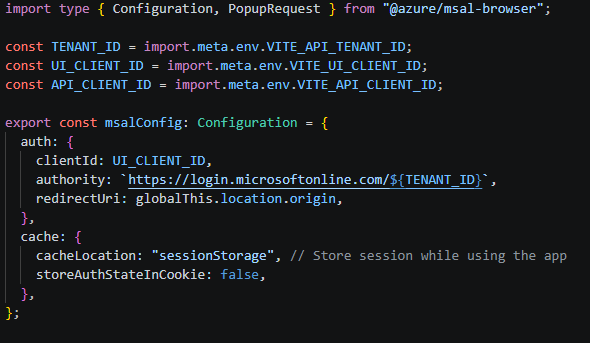
\includegraphics[width=0.6\textwidth]{Images/Implementation/ClientIdTenantId.png}
    \caption[MSAL configuration in authConfig.ts]
    {MSAL configuration in \texttt{authConfig.ts}. [Own creation]}
    \label{fig:auth-config}
\end{figure}

\vspace{-0.5cm}

To ensure the authentication is applied throughout the entire application, the root React component is wrapped with the \texttt{MsalProvider} in the main entry point file (\texttt{main.tsx}), as configured in Figure \ref{fig:msal-provider}.


\begin{figure}[H]
    \centering
    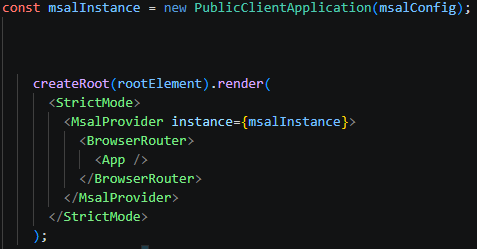
\includegraphics[width=0.6\textwidth]{Images/Implementation/MsalWrappingMain.png}
    \caption[MSAL authentication setup in main.tsx]
    {MSAL authentication setup in \texttt{main.tsx}. [Own creation]}
    \label{fig:msal-provider}
\end{figure}

\vspace{-0.5cm}

An Axios interceptor is also implemented in the \texttt{apiClient.ts} file to automatically secure communication with the backend API. This small piece of code intercepts every outgoing API request, silently acquires a valid JWT access token from MSAL, and adds it to the \texttt{Authorization} header. In this way, every API request is authenticated while avoiding repetitive code in each component. The detailed code implementation is provided in Figure \ref{fig:api-client}.


\begin{figure}[H]
    \centering
    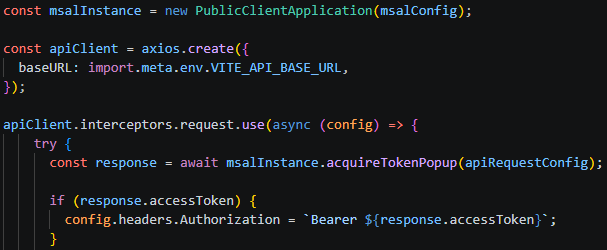
\includegraphics[width=0.7\textwidth]{Images/Implementation/apiClient.png}
    \caption[Axios interceptor configuration in apiClient.tsx]
    {Axios interceptor configuration in \texttt{apiClient.tsx}. [Own creation]}
    \label{fig:api-client}
\end{figure}



